\subsubsection{Strategies and metrics}
\label{sub:strategies_and_metrics}

This subsection will list and describe important metrics, heuristics and design choices that are either fundamentally important for deep learning or that will be used throughout this work.

\paragraph{Optimization}
Optimization algorithms form the foundation of learning in \gls{nn}s. The goal is to minimize the loss function (paragraph~\ref{par:cost_function}) through best possible parameter updates. Paragraph~\ref{par:backprop} introduced a basic structure for optimization algorithms in \gls{nn} training as well as update functions for the \textit{\gls{sgd}} optimization algorithm. To improve readability throughout the rest of the paragraph, the previously presented weight update rule (equation~\ref{eq:backprop_five}) is shown again in equation~\ref{eq:basic_update} in a slighly modified form.
\begin{equation}
	\label{eq:basic_update}
	\theta_{i+1} = \theta_{i} - \alpha \nabla f(\theta_i)
\end{equation}
However, with more complicated and multi-dimensional loss functions, traditional gradient descent methods struggle at converging towards optimal global minima. \gls{sgd} especially has trouble navigating through ravines, i.e. areas where the surface curves much more steeply in one dimension than in another, which are common around local optima. As a countermeasure to this problem, researchers found inspiration in the field of physics - a ball that is rolling down a very steep slope will have a higher \textit{velocity} than one that is rolling down a fairly flat slope. From this insight stems the concept of \textbf{momentum} in numerical optimization developed in the 1960s~\footcite{10.5555/3042817.3043064}. In its essence, momentum can be seen as a moving average of the gradients that helps accelerate optimization in the right directions, thus leading to faster converging. It can especially help reduce oscillations in `ravine'-like settings that would otherwise slow down the gradient descent algorithm and prevent us from using a large learning rate. The way momentum works is through remembering the discounted past gradient steps, then adding the current one with a certain learning rate to it in order to get a mixture of both.
\begin{align}
	v_{i+1} &= \gamma v_i + \alpha \nabla f(\theta_i) \label{eq:velocity_update} \\
	\theta_{i+1} &= \theta_i - v_{i+1} \label{momentum_update}
\end{align}
Equation~\ref{eq:velocity_update} demonstrates calculation of the weight update, or \textit{velocity}, $ v_{t+1} $ which consists of two terms: the gradient $ \nabla f(\theta_i) $ weighted with the learning rate $ \alpha $, and the previous update/velocity $ v_t $ multiplied by the \textit{momentum constant} $ \gamma $. This discounting factor $ \gamma $ is a hyperparameter and it basically tells us how much to remember from past gradients. The nature of this calculation leads to having stronger updates when gradients are scoring high absolute values and weaker updates when gradients are scoring lower absolute values. Momentum allows the optimizer to progress more evenly without too many changes of direction (figure~\ref{fig:momentum}).

The perhaps most used optimizer, especially in deep learning, is called \textbf{\gls{adam}}~\footcite{kingma2014adam} and builds on the concept of momentum. Equations \ref{eq:adam_one} through \ref{eq:adam_six} illustrate the computation sequence for a parameter update of $ \theta $ in step $ i $.
\begin{align}
	g_i &= \nabla f(\theta_i) \label{eq:adam_one} \\
	m_i &= \beta_1 m_{i-1} + (1 - \beta_1) g_i \label{eq:adam_two} \\
	v_i &= \beta_2 v_{i-1} + (1 - \beta_2) g_i^2 \label{eq:adam_three} \\
	\hat{m}_i &= \frac{m_i}{1  - \beta_1^i} \label{eq:adam_four} \\
	\hat{v}_i &= \frac{v_i}{1 - \beta_2^i} \label{eq:adam_five} \\
	\theta_{i+1} &= \theta_i - \frac{\alpha}{\sqrt{\hat{v}_i + \epsilon}} \hat{m}_i \label{eq:adam_six} 
\end{align}
Equations \ref{eq:adam_two} and \ref{eq:adam_three} compute mean and uncentered variance estimates of the gradient, similar to momentum. The weighting of the previous estimators is described by the hyperparameteres $ \beta_1 $ and $ \beta_2 $. Since $ m_i $ and $ v_i $ are initialized as zero vectors, they are quite small, especially during the first training steps. In equations \ref{eq:adam_four} and \ref{eq:adam_five} these distortions are counteracted by the calculation of the corrected estimators $ \hat{m}_i $ and $ \hat{v}_i $. The corrected moments are used to update the parameters in equation~\ref{eq:adam_six}. The addition by $ \epsilon $ is done in order to prevent a division by zero. \gls{adam} combines the advantages of two widely used optimization methods: the ability of \textit{AdaGrad} to handle low-value gradients and the ability of \textit{RMSProp} to handle transient targets.  Further advantages of the method are the simple implementation, computational efficiency and the relatively low memory requirements. Therefore, the algorithm as well as different variations, such as \textit{AdaMax} and \textit{Nadam}~\footcite{dozat2016incorporating}, are frequently used in newer language models~\footcite{nyamen2018improveadam}.

\begin{figure}
	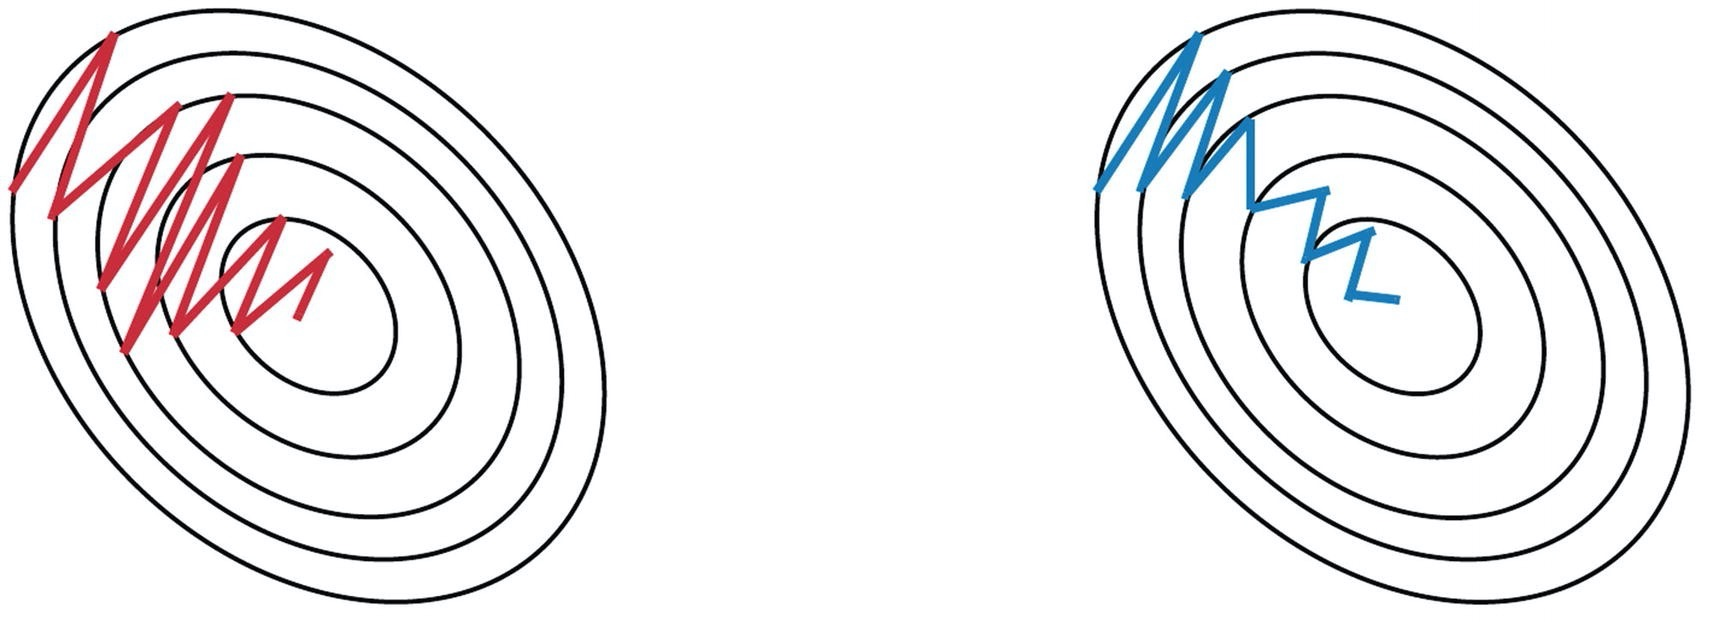
\includegraphics[height=4cm]{img/momentum}
	\caption{Stochastic gradient descent without (left) and with (right) momentum}
	\label{fig:momentum}
\end{figure}

\paragraph{Sampling strategies}
For tasks like text generation, where we receive a probability distribution over words, we have to decide how we are going to select the actual word that our model is going to predict. Simply selecting the one with the highest probability will likely end up in very repetitive behavior (``I don't know. I don't know. I don't know...''), so more sophisticated methods are employed. In this paragraph three of the most impactful and widely used strategies will shortly be presented. \textbf{Top-k} sampling simply samples from the top $ k $ probable words, zero-ing the probabilites for anything below the $ k^{th} $ token. Top-k sampling is often confronted with its inability to dynamically adapt the parameter $ k $. A more powerful version of top-k sampling is \textbf{beam search} decoding. Here, we keep a track of the $ k $ most probable tokens after each step, building up a tree structure (with each node having $ k $ children) until we reach the end of a sequence (marked by an \textit{<END>} token), and at the end we select the path, or \textit{`hypothesis'}, with the highest overall probability. This allows for more coherent sentence structures than top-k sampling as whole sentences are taken into consideration and not only single words. In some cases, though, there is a wide range of words that could reasonably be sampled from (larger $ k $ would be more suited) while in other cases there is only a narrow distribution that can practically be considered (here a smaller $ k $ would be better suited). This limitation, which occurs in both methods metioned above, is addressed by \textbf{top p} (or \textbf{nucleus}) sampling~\footcite{DBLP:journals/corr/abs-1904-09751}: Instead of sampling from the best $ k $ tokens, we sample from those tokens that cumulatively add up to a probability of $ p $. The parameter $ p $ is hereby usually set at a value of around $ 0.9 $. Through this approach, we still avoid sampling `wrong' tokens, but preserve variety when the highest scoring tokens have only small confidence scores.

\paragraph{Regularization}
Deep \gls{nn}s can contain thousands, millions and sometimes even billions of paramteres. In most cases, the datasets used to train these models have far fewer datapoints than the network has weights. In that sense, \gls{nn}s are prone to overfit (i.e. performing well on training data but not adapting well to test data from the same underlying distribution). To prevent this behavior, there are a few possibilites. One is to stop the training earlier, e.g. when the validation error starts rising again. Another powerful technique is \textbf{regularization}. In the following, two common regularization techniques will be described. \textbf{Dropout}~\footcite{JMLR:v15:srivastava14a} regularization is frequently used because of its simplicity, universality and effectiveness. Dropout forces the \gls{nn} to focus more effectively on the relevant neurons and prune out others. This is accomplished by zero-ing out weights intermittently and letting only a subset of neurons predict the output. Consequently, the units in the \gls{nn} can not co-adapt too much and the model has to generalize its structure. The implementation of Dropout is simple and straightforward:
\begin{align}
	a_i = f_i (z) d_i \qquad \text{with} \ \ d_i \in \{0, 1\} \ \ \text{and} \ \ p(d_i = 1) = p_{\text{dropout}}
\end{align}
For each neuron, the decision whether it fires or not depends on not only the activation function $ f_i $, but also on the dropout value $ d_i $ which is either $ 1 $ with a probability of $ p_{\text{dropout}} $ or $ 0 $ else. Another commonly deployed regularization strategy, especially in classification tasks (cross entropy loss, see paragraph~\ref{par:cost_function}), is \textbf{label smoothing}~\footcite{DBLP:journals/corr/abs-1906-02629}. This method first converts the representation of the output $ y $ from a unrestricted vectorspace representation to a distributional vector. This reduces the problem of having `one-hot'-like encoded labels that make the model less adaptive and too confident on its predictions through the large logit gaps. The distributional vector is the result of
\begin{equation}
	y_{\text{smooth}} = y_{\text{hot}} - \alpha * \left( y_{\text{hot}} - \frac{1}{N_c} \right),
\end{equation}
where $ N_c $ is the number of classes and $ \alpha $ is a parameter that determines the amount of smoothing. Selecting $ \alpha = 1 $ returns a uniform distribution while the opposite ($ \alpha = 0 $) returns the original vector. Apart from dropout and label smoothing, there are many other regularization techniques such as punishing weights that are too high (L1 and L2 regularization or soft weight sharing), but these will not be further here as these are computationally rather expensive and are usually found on smaller models.

\paragraph{Normalization}
Normalization techniques are responsible for making training of \gls{nn}s much faster. One common problem found when training \gls{nn}s is the ``covariate shift''~\footcite{DBLP:journals/corr/IoffeS15}, or the change in the distribution of the input values. For instance, if our input data would consist of pictures of the same objects, but on the one hand taken on a webcam and on the other hand taken on a smartphone camera, their distributions would differ. This would lead to layer activations changing over the course of many iterations. Classically, this was problem was handled by lowering the learning rate which in turn leads to slower network training. \textbf{Batch normalization} addresses this problem by normalizing layer inputs for a mini-batch of examples in an iteration. To achieve this normalization $ \widetilde{x}_i $, inputs $ x_i $ are normalized across the mini-batch by subtracting the mean $ \mu_i $ and dividing by the square root of the variance $ \sigma_i^2 $:
\begin{equation}
	\widetilde{x}_i = \frac{x_i - \mu_i}{\sqrt{\sigma_i^2 + \epsilon}}
\end{equation}
The constant $ \epsilon $ is usually added to the denominator to avoid dividing by $ 0 $ or values that are too small. Results have shown that when using batch normalization in a network a less extensive use of dropout is required to achieve the same results. \\
While batch normalization normalizes the input characteristics over the batch dimension, \textbf{layer normalization}~\footcite{ba2016layer} normalizes the inputs over the values of a training set. Layer normalization calculates mean values and variances over each value in the training set, is independent batch sizes, and allows calibration with the moments in each layer. Authors of the original paper found that this easier to use and more straightforward approach to normalization was very effective at stabilizing the hidden state dynamics of recurrent neural networks. Furthermore, they emprirically showed that training time was reduced substantially in different experiments compared with previously published techniques, including batch normalization. Layer normalization can be found in many current \gls{nlp} algorithms.

\paragraph{Perplexity}
Perplexity has its origins in the field of information theory and is a way of measuring how well a probability distribution or a probability model predicts a sample~\footcite{10.2307/24980838}. Basically, it is a different way of displaying the entropy of a system. Because in \gls{nlp} language models ultimately represent a probability model (subsection~\ref{sub:foundations_of_language_modeling}), perplexity is regularly used as a standard evaluation metric (in most \gls{nlp} benchmark tasks, models are evaluated based on perplexity). It can be calculated through
\begin{equation}
	\label{eq:perplexity}
	\text{perplexity} = \prod_{t=1}^{T} \left( \frac{1}{P_{\text{LM}}(x^{(t+1)} | x^{(t)}, \dots, x^{(1)})} \right)^{1/T} = 2^{H(p)}
\end{equation}
\begin{equation}
	H(p) = - \sum_{t=1}^{T} p(x^{(t)}) \ \text{log}_2 \ p(x^{(t)})
\end{equation}
where $ T $ is the number of words in the corpus. The last section of equation~\ref{eq:perplexity} was appended to show the relationship between entropy ($ = H(p) $) and perplexity. As in language modeling perplexity depicts the inverse probability of a corpus according to the \gls{lm}, the lower the perplexity is, the better. However, even though perplexity captures how powerful a \gls{lm} is, it is not directly a metric for how well it performs at \gls{nlp} tasks such as text generation (e.g. if the elected decoding algorithm is suboptimal, perplexity is unaffected). Finally, it should be noted that while perplexity and entropy essentially mean the same thing, perplexity has established itself as the standard metric simply because its results are easier to interpret than those of entropy - to make this tangible one might look at a 6-faced balanced die. The entropy of this die is $ \approx 2.58 $ (3 bits are needed to code a dice roll), while the perplexity is $ 6 $ (perplexity can be seen as `the number of choices' of a random variable).

\paragraph{Transfer learning and fine-tuning}
Currently, for many machine learning tasks, more computing power seems to lead predictably to better performance, and is often complementary to algorithmic advances. This is a statement that has never been so true as it is now. Consequently, training a current state-of-the-art model requires signficant hardware and data resources. While most available \gls{nlp} models ten years ago could be developed and trained with commercial laptops or servers, nowadays much specialized hardware in form of GPUs and TPUs is needed (although research for fast CPU algorithms is conducted as well~\footnote{\url{https://hothardware.com/news/researchers-slide-algorithm-cpu-ai-training-outperforms-gpu}}). One way to face this challenge and still achieve high performance results is through the field of sequential \textbf{transfer learning}, where tasks are learned successively. Transfer learning allows models to be trained for similar tasks or domains to increase their generalization capabilities. This can then lead to models achieving better results in areas outside of their initial specification. Sequential transfer learning comprises two phases: During the \textit{pretraining} phase, the model is trained to learn very general representations for a source domain. Afterwards, in the \textit{adaptation} phase, the model is specifically trained to perform well on a (usually more narrow) target domain. This adaptation, or fine-tuning, phase introduces a minimal set of task-specific parameters for subsequent tasks. In contrast to the transfer learning approach, classical models perform isolated learning of a single prediction model for a certain task - this is mainly suitable for well-defined, narrow tasks and requires training of the model from scratch. \\
Pretraining of \gls{lm}s has proven to be an effective method for improving many \gls{nlp} tasks~\footcite{DBLP:journals/corr/abs-1801-06146}. This shift also allows for an efficient and resource-saving adaptation to the target task while at the same time maintaining (or increasing) performance. Another advantage is that the development of \gls{nlp} systems is accelerated by more easily reusable and better-known systems.
